\documentclass[../main.tex]{subfiles}
\graphicspath{{\subfix{../images/}}}

\begin{document}

% {{{ Motivation
The \uav is one of the most promising enabling technologies in the 
21\textsuperscript{st} century. It has been estimated that
there will be as high as \SI{1.2}{million} \uavs in use 
by 2040~\cite{Amo19}. 
Commonly known as drone, 
it improves many existing applications and makes possible 
innumerable new ones. It can be used to monitor livestock, 
carry out security surveillance, manage traffic 
and discover wildlife.
In addition, it can facilitate search and rescue missions,
aid in military operations and expedite final mile delivery.
This is because the \uav combines the best of both worlds
of satellites and \csns such as \cctvs.
While a fixed \textsc{cctv} is good at taking 
high resolution images and a far away satellite can monitor
large areas, a \uav can do both equally well without 
being restricted in location or image quality. 
In marine biology for instance,  
the study of interactions between members of a migrating 
pod of whales can be done using a \uav but not 
\textsc{cctv}s or satellites.
However, micro-drones, which are the most common type of \uavs,
suffer from limited flight time~\cite{Sha19}. 
This is especially disadvantageous in
the mentioned tasks because they require visitation of targets
whose pattern of movement is the only known information.
% }}}

\subsection{Problem statement}

% {{{ Problem statement
More often than not, individuals and organizations face the problem
of visiting a set of destinations in the fastest time 
possible.
For example, an operation engineer needs to monitor
a number of reactors and plants within his or her shift.
The need to do so in the shortest time can be due to restrictions on
cost, energy or other limited resources of concern.
This problem is commonly known as the travelling salesman problem
where historically, a salesman had to make a decision in order
to visit a set of cities exactly once to conduct his trade
in the most time-saving manner.
Depending on the metric of interest, 
the destinations have to be visited in the correct order.
Algorithms, such as Dijkstra's, have been used 
to find the shortest path between the cities.
However, in applications where the \uav with a limited
flight time is used to 
visit targets which are mobile, the problem is intensified.
As illustrated in \cref{fig:problem}, in order to propose a solution for this problem, this study asks the following question: 
Given the mobile targets' mobility pattern,
how do we make a \uav able to visit them
in the fastest possible time and, in turn, 
the most energy-saving way although it does not know the targets'
exact locations?  
% }}}

% {{{ Figure of the problem
\begin{figure}[tb] 
    \centering
    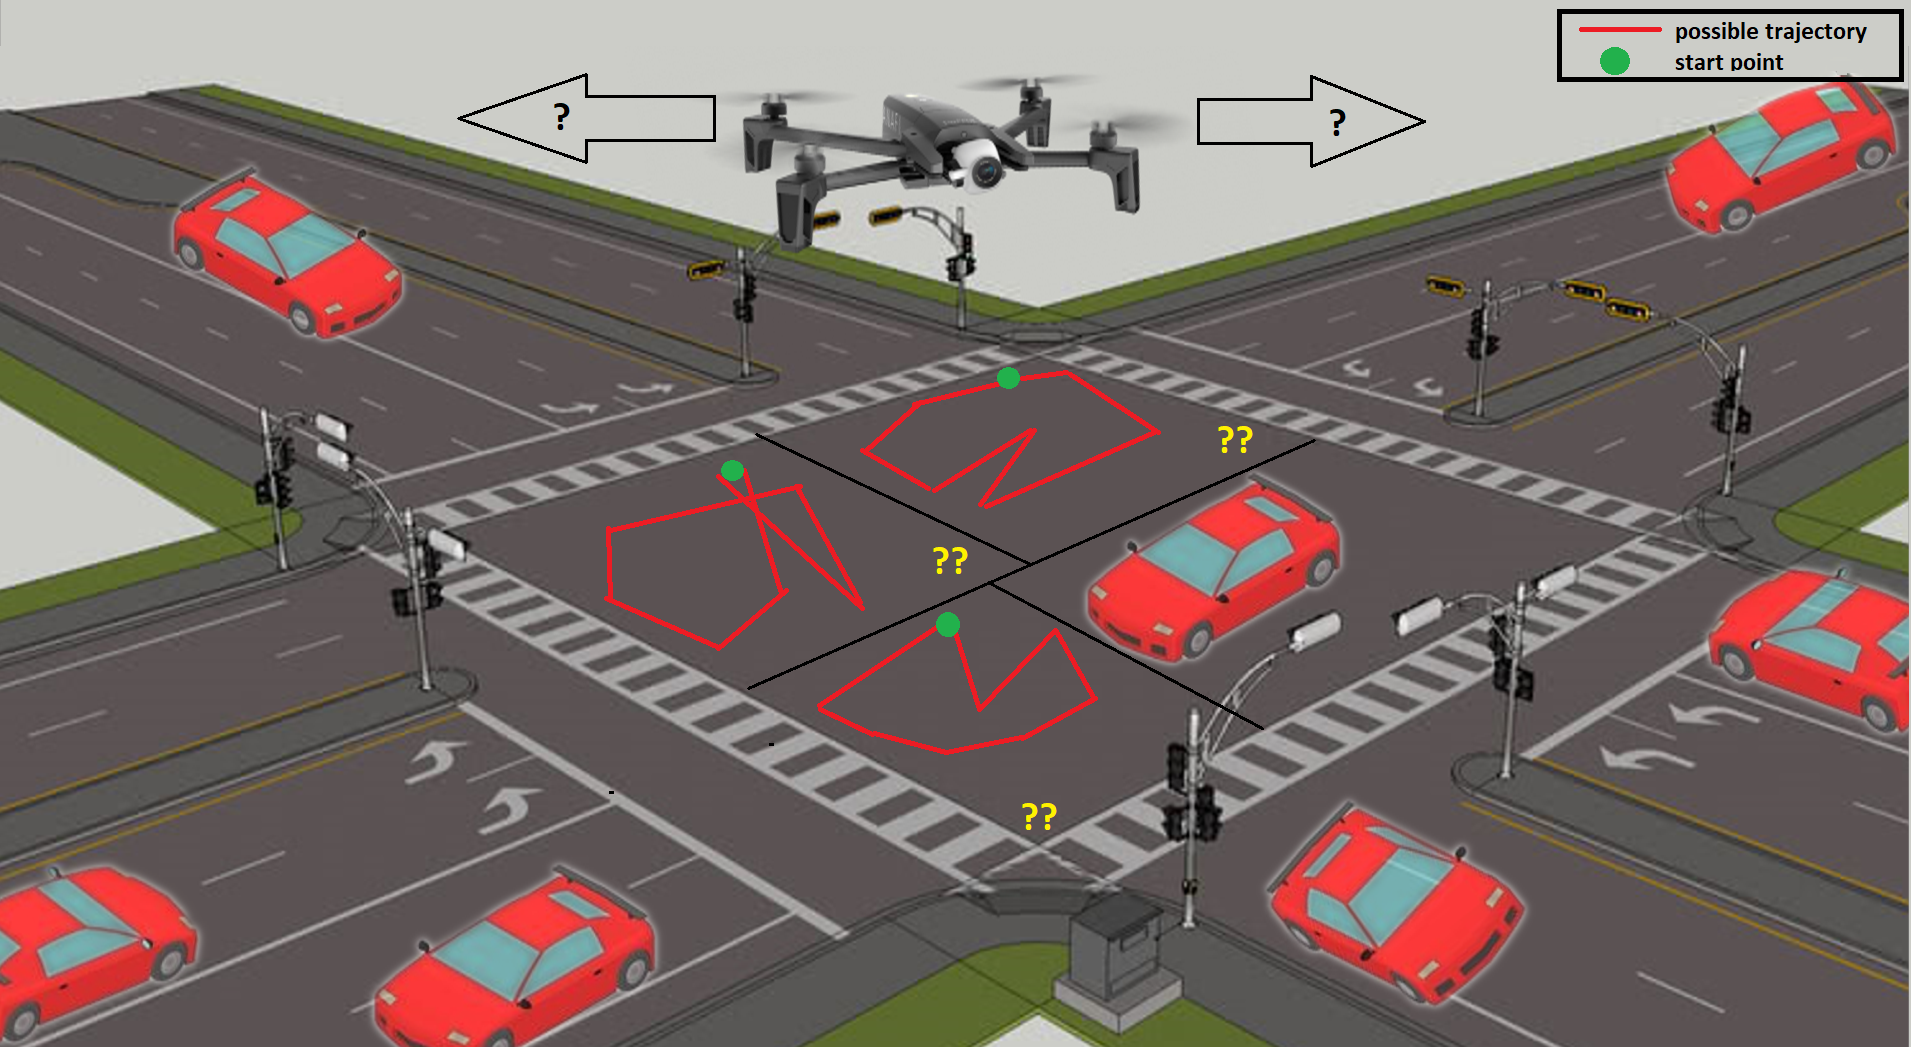
\includegraphics[width=0.9\textwidth]{problem.png} 
    \caption{The \gls{uav} needs to calculate 
    the best trajectory to cover the red cars
    based on their expected movements
    as fast as possible before it runs out of battery.} 
    \label{fig:problem} 
\end{figure}
% }}}

% {{{ Technical and non-technical challenges
There are many inherent challenges that this problem
poses. First of all, it is difficult to make a drone
fly autonomously to visit multiple targets whose locations
have not been known beforehand. 
Not only that the targets must be detected, 
but they also need to be uniquely
identified so that the already visited targets
can be distinguished from those that have not been visited.
This is a common scenario in various applications. 
Moreover, this needs to be done in the minimum
amount of flight time because \uavs use batteries
as their main power supply.
Otherwise, several units need to be used concurrently
or sequentially.
Secondly, flying a drone efficiently is complicated 
because it has six degrees of freedom. In other words, 
there are many parameters that the controller needs to 
take into account to move 
it precisely to a destination point. 
Thirdly, there will be obstacles that the autonomous \uav
needs to know how to avoid while visiting the targets.
Last but not least, the fact that \uavs communicate wirelessly
with the command and control station in the open 
over a long range makes them susceptible
to malicious hackers.
Based on the goal of the project, the main challenge 
that we focused on is the autonomous navigation
of the drone to visit identifiable and mobile targets in the shortest
time and energy-saving way.
% }}}

% {{{ Solution
From a high level, the solution will involve machine learning
to uniquely identify the targets, and reinforcement learning
to make the drone autonomously visit the targets in the
shortest time possible. In addition, there will also be
a hardware integration between a drone and an onboard
computer. This is to avoid the command and control
station sending the frequent low-level commands to control
the drone's propellers. 
Instead, the drone
will possess its own computer that it will use to 
autonomously visit the targets.
% }}}

\subsection{Project significance}

% {{{ Project importance
The significance of the project is enormous. 
Making a \uav able to intelligently 
visit mobile targets in the shortest time
and minimal mechanical energy 
opens doors to many existing and new applications
due to the \uav's unique features.
First of all, the \gls{uav} combines the best features
from \textsc{cctv}s and satellites.
Using \glspl{uav} gives the benefit of high resolution images
for the purposes of surveillance and monitoring
similar to \textsc{cctv} cameras 
without the restriction in movement~\cite{Sha19}.
At the same time, it allows for large-scale monitoring 
usually done exclusively using satellites 
without its low accuracy~\cite{Sha19}.
This feature of the \uav is useful in applications
such as marine biology, livestock monitoring and military
reconnaissance.
Second of all, target visitation done by a \gls{uav}
is faster compared to terrestrial vehicles
because it has a higher degree of freedom, and
flying at a higher altitude 
allows it to avoid 
many of the surrounding obstacles.
This makes it more suited for traffic monitoring and last mile delivery
among others. In the long term, we hope to see \uavs helping the
blind to visit particular destinations or acting as first
responders to crash sites and crime scenes.
% }}}

% {{{{ Describe how can stakeholders use the project,
% ## its uses/applications,
% ## impacts if the design problem was not solved,
% ## and benefits of the project in Qatar and the region.
Based on the project's significance, we have identified 
its stakeholders to be 
those companies, institutions and organizations which
have certain fixed or mobile subjects of interest 
that they want to monitor, capture or track.
By using our proposed solution,
they will be able to make the aforementioned applications
a reality.
On the other hand, the absence of this project will mean that
they will remain
time-consuming, tedious and expensive
while some will remain infeasible
causing the stakeholders to be deprived of ample growth opportunities.
In some instances, the difference between using 
and not using an intelligent \gls{uav} 
\gls{drl}-trained on mobile target visitation
will be a matter of life-and-death
such as in the search-and-rescue field.

Moreover, Qatar stands to benefit the most from this project 
considering the \textsc{fifa} 2022 it will be hosting
and its rapidly transforming economy and population.
For example, the use of drones can help manage 
the \textsc{fifa} World Cup 
and the increase in population through better monitoring 
of traffic and people, whose data can contribute
to better studies in those sectors. Such a scenario 
is portrayed in \cref{fig:fifa}.
In addition, the Covid 19 has made online shopping
the number one choice for 
the majority of people to buy goods in Qatar~\cite{Has20}.
The success of this project can help in delivering
the goods to intended destinations with minimum delay,
thus contributing to a healthy economy.
% }}}

% {{{ Figure of benefits to Qatar
\begin{figure}[tb] 
    \centering
    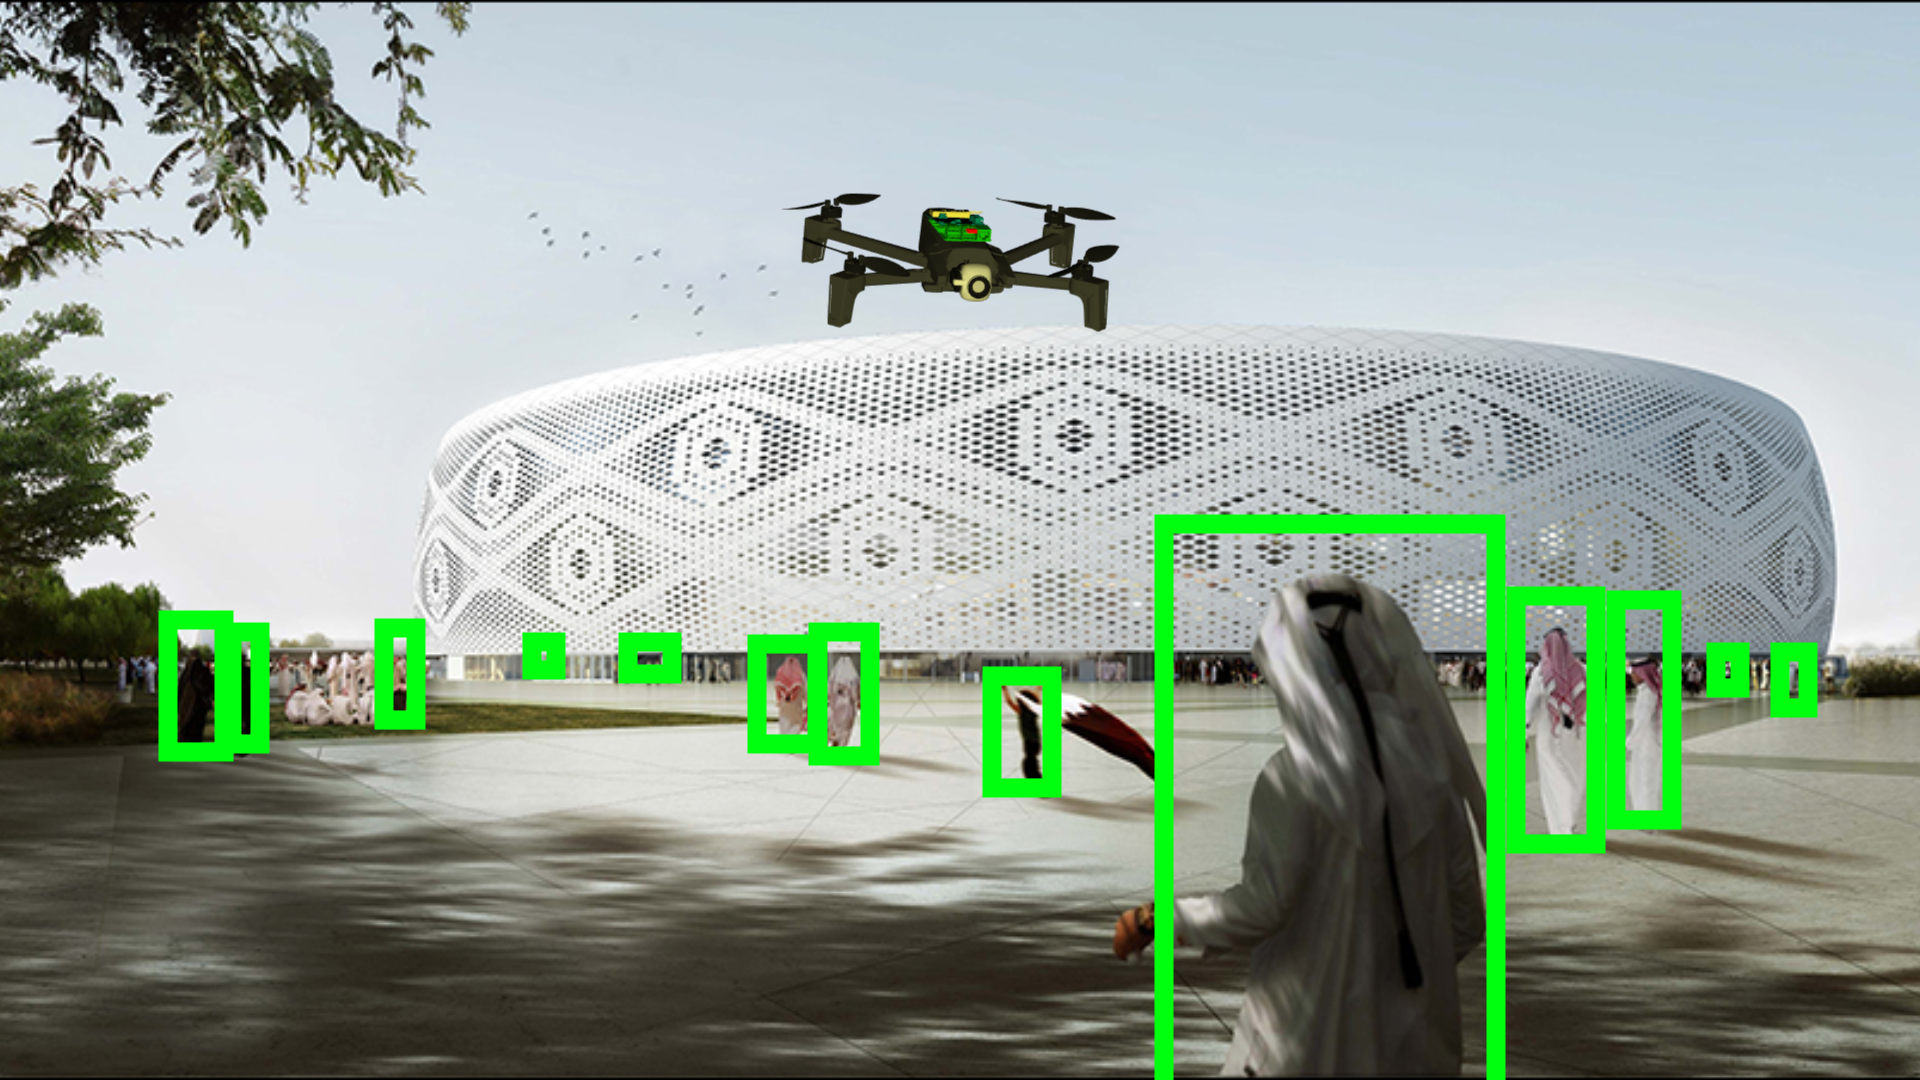
\includegraphics[width=0.9\textwidth]{qatar2022} 
    \caption{The \uav can help prevent misconducts during
    the 2022 \textsc{fifa} World Cup in Qatar by flying 
    over crowded sites to detect potential red flags.} 
    \label{fig:fifa} 
\end{figure}
% }}}

% {{{ Why do you want to do this project? 
% # What got you interested in it? 
% # And how this project will help you further your career goals?
The project significance even extends to the present students
on a personal and individual level.
The prime evidence that has attracted the students to invest
their energy and time in this project is
the increasing number of giant companies like Amazon, Alphabet
and Microsoft experimenting with and profiting from \glspl{uav}
to improve their operations~\cite{Jun17}.
Target visitation is an important subtask of these, among others.
Therefore, we believe there is a huge value
in this project and upon the successful completion of it,
there will be many doors opening to us in terms of
career opportunities because 
this technology is in high demand yet, 
people with the right competency
are scarce.
Besides the jobs that are directly related to the project,
there are other fields that will appreciate the knowledge
and skills that we will gain from the methodological processes 
of designing the simulation,
exploring \gls{drl} and testing them in the real world.
These include robotics, machine learning, and 
network security.
% }}}

\subsection{Project objectives}\label{sec:objectives}

% {{{ Express clear specific objectives
The aim of this project is to create a process 
by which a cyber-physical simulator is used to train 
a \gls{drl} model. This model will then be used
to make a \gls{uav} accurately accomplish a
mobile target visitation task.
The specific objectives of the project are as follows:

\begin{enumerate}
    \item \label{obj:overview}
        To Develop a solution composed of a drone and
        a command and control system which can be used
        to track fixed and mobile targets in the
        minimum amount of flight time
    \item \label{obj:hardware} To Design and integrate 
        hardware to enable 
        intelligence on the drone
    \item To Develop a command and control system that
        is able to provide high-level commands 
        to the drone
    \item \label{obj:machine-learning} 
        To Detect and identify
        targets when they are visited by the drone
        using a pre-trained \gls{ml} model
    \item \label{obj:drl} 
        To Minimize the mechanical energy through efficiently
        navigating the drone by leveraging \gls{rl}
    \item \label{obj:simulation} 
        To Use cyber-physical simulation in the \gls{rl} training
        to teach the drone how to navigate the targets
        intelligently, and test the navigation in a realistic
        3D environment before the actual deployment
\end{enumerate}
% }}}

% {{{ Deliverables and desired results
To demonstrate the objectives, there will be a number 
of deliverables that we will produce.
Firstly, we will present a detailed report 
that will elaborate on our aim, objectives, 
literature review, methodology,
solution and the market value of the project.
Secondly, we will output a trained \gls{drl} model for 
the target visitation task based on a specific
mobility pattern.
Finally, we will build a \gls{uav} system
consisting of the \anafi drone as well as a Raspberry Pi
that will utilize the machine learning and reinforcement learning
models making the \anafi drone fully autonomous.
Based on the deliverables, the desired result is that
given the same mobility pattern for 
the moving targets,
the \gls{uav} should be able to fly to locations it has learned
that will allow it to capture the maximum number of targets in the
shortest time possible. 
% }}}

\subsection{Market research and business viability}

\documentclass[../main.tex]{subfiles}

\begin{document}
\subsection{Business products}
        Technology and \textsc{ai} advancements have been changing human lives for the better.
	The possible opportunities for innovation and creativity are unlimited, this
	project has many aspects that could lead to business opportunities and commercial
	prototypes. 
	One of the many commercial products that could come out of this project is
	the \gls{drl} object detection model. This model can be used in any system
	that requires object detection, it could be a \gls{uav}, a \textsc{cctv} camera, or
	any system that inputs an image to the model after being trained on a similar 
	data set.
	Depending on the system, the \gls{drl} model could be trained using a different
	data set to detect a different object (e.g. cars, humans, animals).
	Another possible product is the \gls{drl} model responsible for navigating the
	drone after being trained on a specific movement pattern.
	Moreover, The entire system developed in this project is a viable product.
	
	According to \citeauthor{Atwater15Commercial}, the global market of drones is 
	increasingly becoming a key player in both military and civilian applications.
	The net value of the \glspl{uav} industry is estimated to reach 13 billion dollars
	by 2024, this is due to the efficiency and flexibility of \glspl{uav} in completing 
	various tasks.
	
	\begin{figure}[H] 
		\centering
		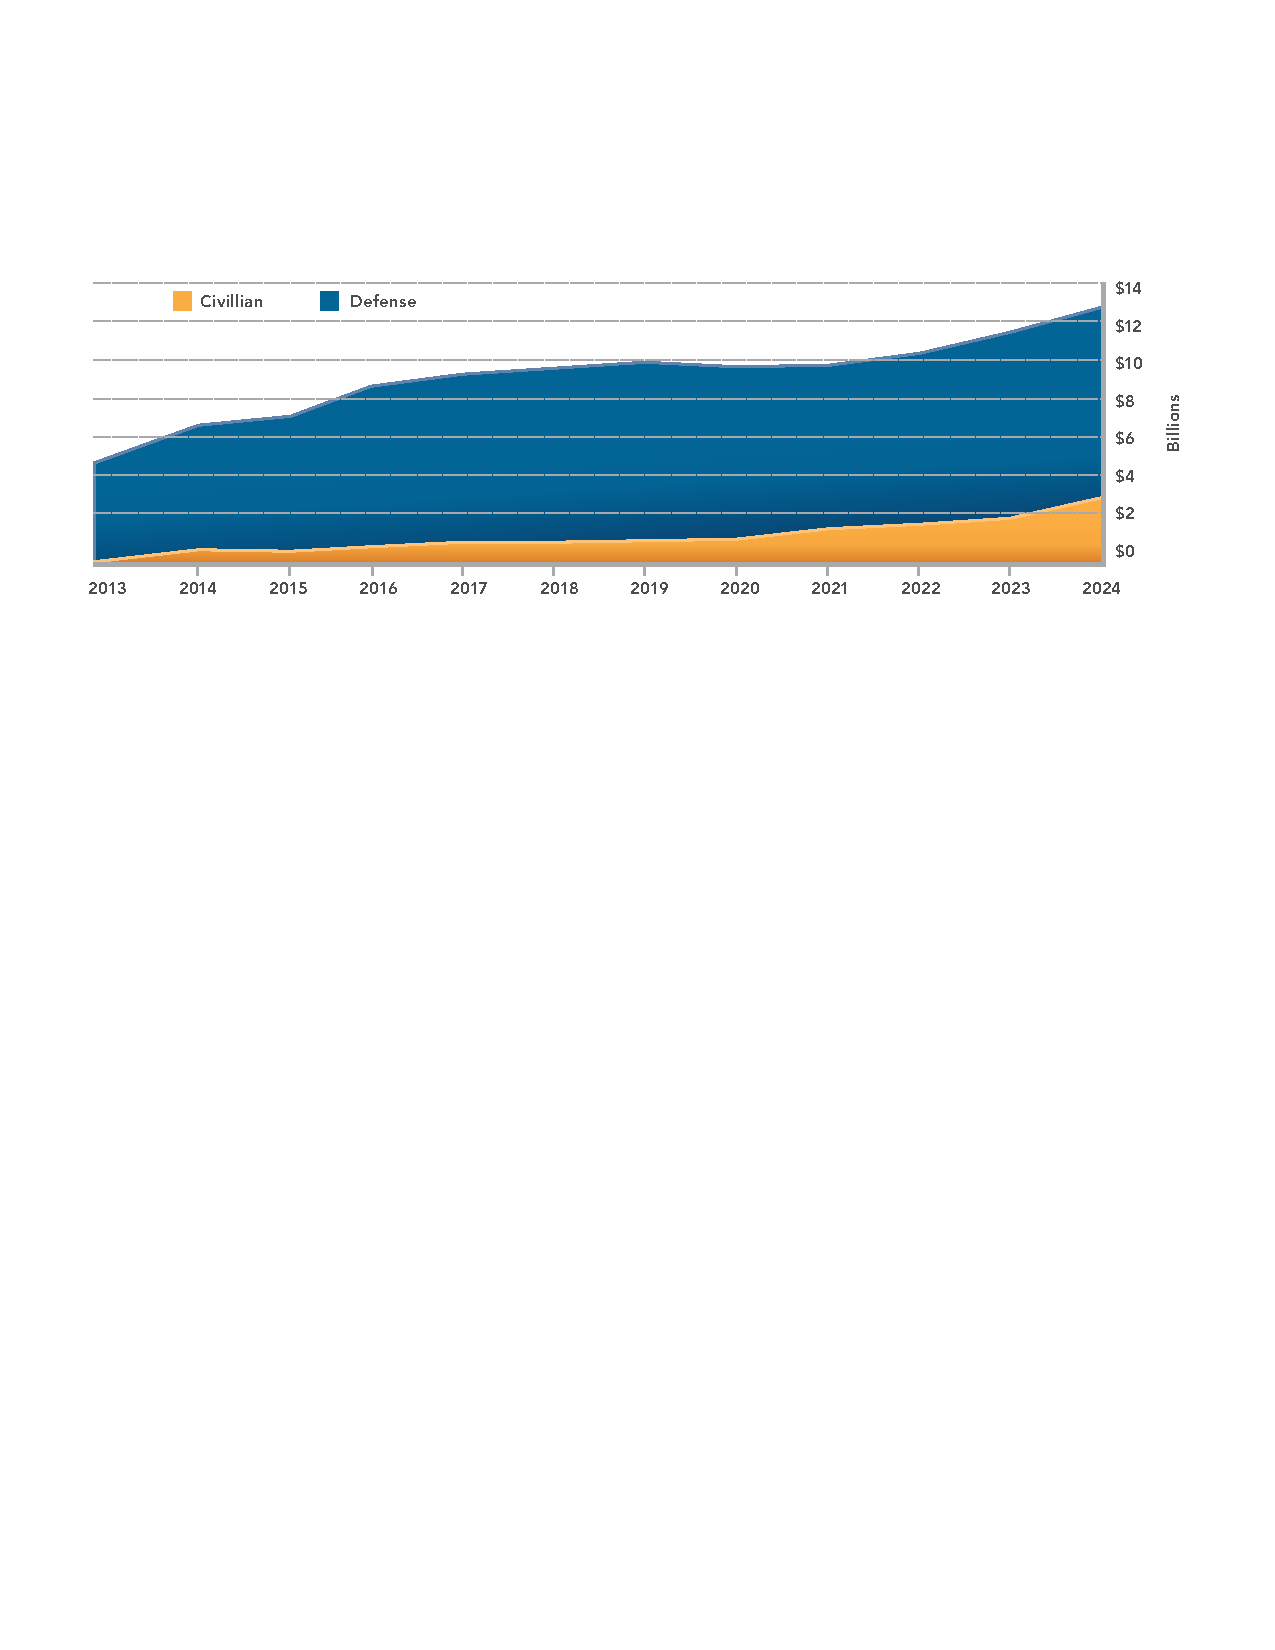
\includegraphics[width=0.65\textwidth, height=6.5cm]{drone-market} 
		\caption{Global drone market} \label{fig:drone-market} 
	\end{figure}
	
	
\subsection{Interested parties}
	Many companies and stakeholders would be interested in acquiring either the
	complete system that we produce, or sub-parts (e.g. \gls{drl} model)
	\begin{enumerate}
		\item Military applications: Drones and object detection models could 
		be used in military operations to detect people of danger, secure 
		sensitive areas, and even eliminate threats (i.e. drone weaponry).
		
		\item Biological research institutes, the \gls{uav} along with the object
		detection model that we provide could be trained to detect certain animals 
		and track them, this would revolutionize biological research.
		
		\item Security companies, personal home security could be established through
		\glspl{uav} and such object detection models could detect threats or unusual
		behaviors. This is applicable in any public area or even personal properties.		
		
	\end{enumerate}

\subsection{Viability in Qatar}
	Our product is simple enough to be used by anyone, however it is mostly intended for 
	authorized institutes that have a license to fly \glspl{uav} as the legal limitations 
	in the region are very strict. 
	A lot of the possible applications are for out of town use (e.g. biological research), 
	this makes the product more acceptable to the public as it does not invade anyone's privacy.
	Moreover, one of the major advantages for our product is that there are no competitors 
	inside Qatar, most drones in Qatar are used for photography purposes, and our
	specific product idea has never been deployed in Qatar, so this gives us an excellent 
	market headstart and implies the huge market need for such products.
\subsection{Product Price}
To choose an acceptable price, we must analyze the different components of the system. Their prices are listed in the \cref{tab:components-prices} below:
	\\
	\begin{table}[H]
		\begin{center}
			\caption{A price list of the system components.}
			\label{tab:components-prices}
			\begin{tabular}{p{3.5cm} c c} 
                            \toprule
                            \textbf{Component} & \textbf{Price(\$)} & \textbf{Price(\textsc{qr})}\\
				\midrule
				\anafi Drone & 800.00 & 2920.00 \\
				Raspberry Pi & 150.00 & 547.50 \\
				Raspberry Pi battery & 30.00 & 109.50\\
				Wi-Fi Dongle & 20.00 & 73.00\\
				\hline 
				Total & 1000.00 & 3650.00 \\
				Selling price & 1644.00 & 6000 \\ 
				Profit/unit & 644.00 & 2350 \\
				\bottomrule
			\end{tabular}
		\end{center}
	\end{table}

	The discussed prices might not be acceptable by individuals, but the product is mainly made for big organizations who certainly can afford the product.
	



\end{document}


\end{document}
